Learning from interactions with users is ubiquitous in modern customer-facing systems, from product recommendations to web search to spam detection to content selection to fine-tuning the interface. Many systems purposefully implement \emph{exploration}: making potentially suboptimal choices for the sake of acquiring new information. Randomized controlled trials, a.k.a. A/B testing, are an industry standard, with a number of companies such as \emph{Optimizely} offering tools and platforms to facilitate them. Many companies use more sophisticated exploration methodologies based on \emph{multi-armed bandits}, a well-known theoretical framework for exploration and making decisions under uncertainty.

%~\cite{KohaviAB-2015,KohaviLSH09}

Systems that engage in exploration typically need to compete against one another; most importantly, they compete for users. This creates an interesting tension between \exploration and \competition. In a nutshell, while exploring may be essential for improving the service tomorrow, it may degrade quality and make users leave \emph{today}, in which case there will be no users to learn from! Thus, users play three distinct roles: they are customers that generate revenue, they generate data for the systems to learn from, and they are self-interested agents which choose among the competing systems.


We initiate a study of the interplay between \exploration and \competition. The main high-level question is: {\bf whether and to what extent competition incentivizes adoption of better exploration algorithms}. This translates into a number of more concrete questions. While it is commonly assumed that better learning technology always helps, is this so for our setting? In other words, would a better learning algorithm result in higher utility for a principal? Would it be used in an equilibrium of the ``competition game"? Also, does competition lead to better social welfare compared to a monopoly? We investigate these questions for several models, as we vary the capacity of users to make rational decisions (\rationality ) and the severity of competition between the learning systems (\competitiveness). The two are controlled by the same ``knob" in our models; \asedit{such coupling is not unusual in the literature, \eg see \citet{Gabaix-16}}.

\asedit{On a high level, our contributions can be framed in terms of the ``inverted-U relationship" between rationality/competitiveness and the quality of adopted algorithms (see \reffig{fig:inverted-U}).}

\OMIT{The relationship between the severity of competition among firms and the quality of technology adopted as a result of this competition is a familiar  theme in the economics literature, known as ``competition vs. innovation".%
\footnote{In this context, \innovation usually refers to adoption of a better technology as a substantial R\&D expense to a given firm. It is not as salient whether similar ideas and/or technologies already exist outside the firm. }
We frame our contributions in terms of the ``inverted-U relationship", a conventional wisdom regarding ``competition vs. innovation" (see \reffig{fig:inverted-U}).}

\begin{figure}
\begin{center}
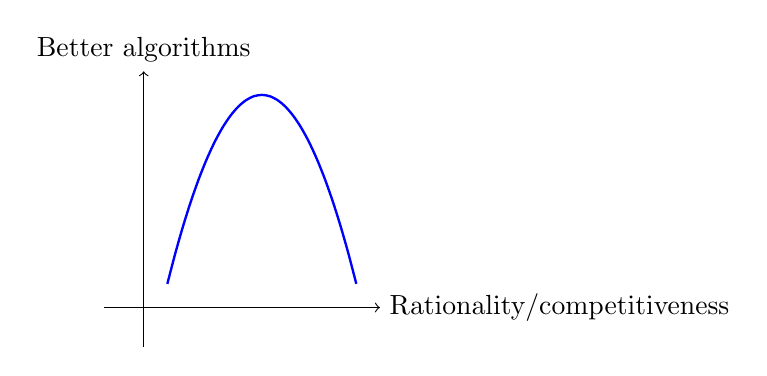
\begin{tikzpicture}
      \draw[->] (-.5,0) -- (3,0) node[right] {Rationality/competitiveness};
      \draw[->] (0,-.5) -- (0,3) node[above] {Better algorithms};
      \draw[scale=0.6,domain=0.5:4.5,smooth,variable=\x,blue, line width=0.3mm] plot ({\x},{4.5 - (\x - 2.5)^2});
      % \draw[scale=0.5,domain=-3:3,smooth,variable=\y,red]  plot ({\y*\y},{\y});
 \end{tikzpicture}

\caption{Inverted-U relationship between rationality/competitiveness and algorithms.}
\label{fig:inverted-U}
\end{center}
\end{figure}



% the extent to which the game between the two principals is competitive
% degree of innovation that these models incentivize.
% the extent to which agents make rational decisions


%\subsection{Our model}
%\label{sec:intro-model}

\xhdr{Our model.} We define a game in which two firms (\emph{principals}) simultaneously engage in exploration and compete for users (\emph{agents}). These two processes are interlinked, as exploration decisions are experienced by users and informed by their feedback. We need to specify several conceptual pieces: how the principals and agents interact, what is the machine learning problem faced by each principal, and what is the information structure. Each piece can get rather complicated in isolation, let alone jointly, so we strive for simplicity. Thus, the basic model is as follows:

\begin{itemize}

\item A new agent arrives in each round $t=1,2, \ldots$, and chooses among the two principals. The principal chooses an action (\eg a list of web search results to show to the agent), the user experiences this action, and reports a reward. \asedit{All agents have the same ``decision rule" for choosing among the principals given the available information.}

\item Each principal faces a very basic and well-studied version of the multi-armed bandit problem: for each arriving agent, it chooses from a fixed set of actions  (a.k.a. \emph{arms}) and receives a reward drawn independently from a fixed distribution specific to this action.

\item Principals simultaneously announce their learning algorithms \asedit{before round $1$}, and cannot change them afterwards. There is a common Bayesian prior on the rewards (but the realized reward distributions are not observed by the principals or the agents). Agents do not receive \asedit{any other information}. Each principal only observes agents that chose him.
\end{itemize}

\xhdr{Technical results.}
Our results depend crucially on agents' ``decision rule" for choosing among the principals. The simplest and perhaps the most obvious rule is to select the principal which maximizes their expected utility; we refer to it as \HardMax. We find that \HardMax is not conducive to \asedit{adopting better algorithms}. In fact, each principal's dominant strategy is to do no purposeful exploration whatsoever, and instead always choose an action that maximizes expected reward given the current information; we call this algorithm \DynGreedy. While this algorithm may potentially try out different actions over time and acquire useful information, it is known to be dramatically bad in many important cases of multi-armed bandits --- precisely because it does not explore on purpose, and may therefore fail to discover best/better actions. Further, we show that \HardMax is very sensitive to tie-breaking when both principals have exactly the same expected utility according to agents' beliefs. If tie-breaking is probabilistically biased --- say, principal 1 is always chosen with probability strictly larger than $\tfrac12$ --- then this principal has a simple ``winning strategy" no matter what the other principal does.

We relax \HardMax to allow each principal to be chosen with some fixed baseline probability. One intuitive interpretation is that there are ``random agents" who choose a principal uniformly at random, and each arriving agent is either \HardMax or ``random" with some fixed probability. We call this model \HardMaxRandom. We find that \asedit{better algorithms} help in a big way: a sufficiently better algorithm is guaranteed to win all \asedit{non-random} agents after an initial learning phase. While the precise notion of ``sufficiently better algorithm" is rather subtle, we note that commonly known ``smart" bandit algorithms typically defeat the commonly known ``naive" ones, and the latter typically defeat \DynGreedy. However, there is a substantial caveat: one can defeat any algorithm by interleaving it with \DynGreedy. This has two undesirable corollaries: a better algorithm may sometimes lose, and a pure Nash equilibrium typically does not exist.

We further relax the decision rule so that the probability of choosing a given principal varies smoothly as a function of the difference between  principals' expected rewards; we call it \SoftMaxRandom. For this model, the ``better algorithm wins" result holds under much weaker assumptions on what constitutes a better algorithm. This is the most technical result of the paper. The competition in this setting is necessarily much more relaxed: typically, both principals attract approximately half of the agents as time goes by (but a better algorithm may attract slightly more).

All results extend to a much more general version of the multi-armed bandit problem in which the principal may observe additional feedback before and/or after each decision, as long as the feedback distribution does not change over time. In most results, principal's utility may depend on both the market share and agents' rewards.

\xhdr{Economic interpretation.}
\asedit{The inverted-U relationship between the severity of competition among firms and the quality of technologies that they adopt is a familiar theme in the economics literature \citep[\eg][]{Aghion-QJE05,Vives-08}.%
\footnote{The literature frames this relationship as one between ``competition" and ``innovation". In this context, ``innovation" refers to adoption of a better technology, at a substantial R\&D expense to a given firm. It is not salient whether similar ideas and/or technologies already exist outside the firm. It is worth noting that adoption of exploration algorithms tends to require substantial R\&D effort in practice, even if the algorithms themselves are well-known in the research literature; see \citet{MWT-WhitePaper-2016} for an example of such R\&D effort.}
We find it illuminating to frame our contributions in a similar manner, as illustrated in \reffig{fig:inverted-U}.

Our models differ in terms of rationality in agents' decision-making: from fully rational decisions with \HardMax to relaxed rationality with \HardMaxRandom to an even more relaxed rationality with \SoftMaxRandom. The same distinctions also control the severity of competition between the principals: from cut-throat competition with \HardMax to a more relaxed competition with \HardMaxRandom, to an even more relaxed competition with \SoftMaxRandom. Indeed, with \HardMax you lose all customers as soon as you fall behind in performance, with \HardMaxRandom you get some small market share no matter what, and with \SoftMaxRandom you are further guaranteed a market share close to $\tfrac12$ as long as your performance is not much worse than the competition. The uniform choice among principals corresponds to no rationality and no competition.

We identify the inverted-U relationship in the spirit of \reffig{fig:inverted-U} that is driven by the rationality/competitiveness distinctions outlined above: from \HardMax to \HardMaxRandom to \SoftMaxRandom to \Uniform. We also find another, technically different inverted-U relationship which zeroes in on the \HardMaxRandom model. We vary rationality/competitiveness inside this model, and track the marginal utility of switching to a better algorithm.

These inverted-U relationships arise for a fundamentally different reason, compared to the existing literature on ``competition vs. innovation.'' In the literature, better technology always helps in a competitive environment, other things being equal. Thus, the tradeoff is between the costs of improving the technology and the benefits that the improved technology provides in the competition. Meanwhile, we find that a better exploration algorithm may sometimes perform much worse under competition, even in the absence of R\&D costs.}

\ascomment{Yishay's edits, slightly edited by Alex}

\xhdr{Discussion.} We capture some pertinent features of reality while ignoring some others for the sake of tractability. Most notably, we assume that agents do not receive any information about other agents' rewards after the game starts. In the final analysis, this assumption makes agents' behavior independent of a particular realization of the Bayesian prior, and therefore enables us to summarize each learning algorithm via its Bayesian-expected rewards (as opposed to detailed performance on the particular realizations of the prior). Such summarization is essential for formulating lucid and general analytic results, let alone proving them. It is a major open question whether one can incorporate signals about other agents' rewards and obtain a tractable model.

We also make a standard assumption that agents are myopic: they do not worry about how their actions impact their future utility. In particular, they do not attempt to learn over time, to second-guess or game future agents, or to manipulate principal's learning algorithm. We believe this is a typical case in practice, in part because agent's influence tend to be small compared to the overall system. We model this simply by assuming that each agent only arrives once.

Much of the challenge in this paper, both conceptual and technical, was in setting up the right model and the matching theorems, and not only in proving the theorems. Apart from making the modeling choices described above, it was crucial to interpret the results and intuitions from the literature on multi-armed bandits so as to formulate meaningful assumptions on bandit algorithms and Bayesian priors which are productive in our setting.

\xhdr{Open questions.}
\asedit{How to incorporate signals about the other agents' rewards? One needs to reason about how exact or coarse these signals are, and how the agents update their beliefs after receiving them. Also, one may need to allow principals' learning algorithms to respond to updates about the other principal's performance. (Or not, since this is not how learning algorithms are usually designed!) A clean, albeit idealized, model would be that (i) each agent learns her exact expected reward from each principal before she needs to choose which principal to go to, but (ii) these updates are invisible to the principals. Even then, one needs to argue about the competition on particular realizations of the Bayesian prior, which appears very challenging.

Another promising extension is to heterogeneous agents. Then the agents' choices are impacted by their idiosyncratic signals/beliefs, instead of being entirely determined by priors and/or signals about the average performance. It would be particularly interesting to investigate the emergence of \emph{specialization}: whether/when an algorithm learns to target specific population segments in order to compete against a more powerful ``incumbent".
} %\asedit


\xhdr{Map of the paper.}
We survey related work (Section~\ref{sec:related-work}), lay out the model and preliminaries (Section~\ref{sec:model}), and proceed to analyze the three main models, \HardMax, \HardMaxRandom and \SoftMaxRandom (in Sections~\ref{sec:rational},~\ref{sec:random}, and ~\ref{sec:soft}, respectively). We discuss economic implications in Section~\ref{sec:welfare}. Appendix~\ref{app:examples} provides some pertinent background on multi-armed bandits. Appendix~\ref{app:perturb} gives a broad example to support an  assumption in our model.




%%% Local Variables:
%%% mode: latex
%%% TeX-master: "main"
%%% End:
